\documentclass[12pt, letterpaper]{memoir}
\usepackage{ExamStyle}

\begin{document}
	\pagestyle{empty}
	\begin{center}
		{\Huge Rowley CHEM 1220 Midterm 3}
	\end{center}
	
	{\large Formulas}
	
	\begin{minipage}{0.5\linewidth}
		$pH=-\log[\ch{H3O^+}]$
		
		$pOH=-\log[\ch{OH^-}]$
		
		$pH + pOH = 14$
		
		$K_aK_b=K_w$
		
		$pK_a=-\log K_a$
	\end{minipage}
	\begin{minipage}{0.5\linewidth}
		$[\ch{H3O^+}] = 10^{-pH}$
		
		$[\ch{OH^-}] = 10^{-pOH}$
		
		$[\ch{H3O^+}][\ch{OH^-}] = K_w=1.00\times10^{-14}$
		
		$pH=pK_a+\log\frac{B}{A}$
		
		$C_AV_A=C_TV_T$
	\end{minipage}
	
	\vspace{2em}

	{\large Constants}
	
	$R=8.314 \dfrac{J}{mol~K}$
	
	$R=0.08206 \dfrac{L~atm}{mol~K}$

	
    \newgeometry{top=1mm, bottom=1mm, left=1mm, right=1mm}


\hspace{6em}	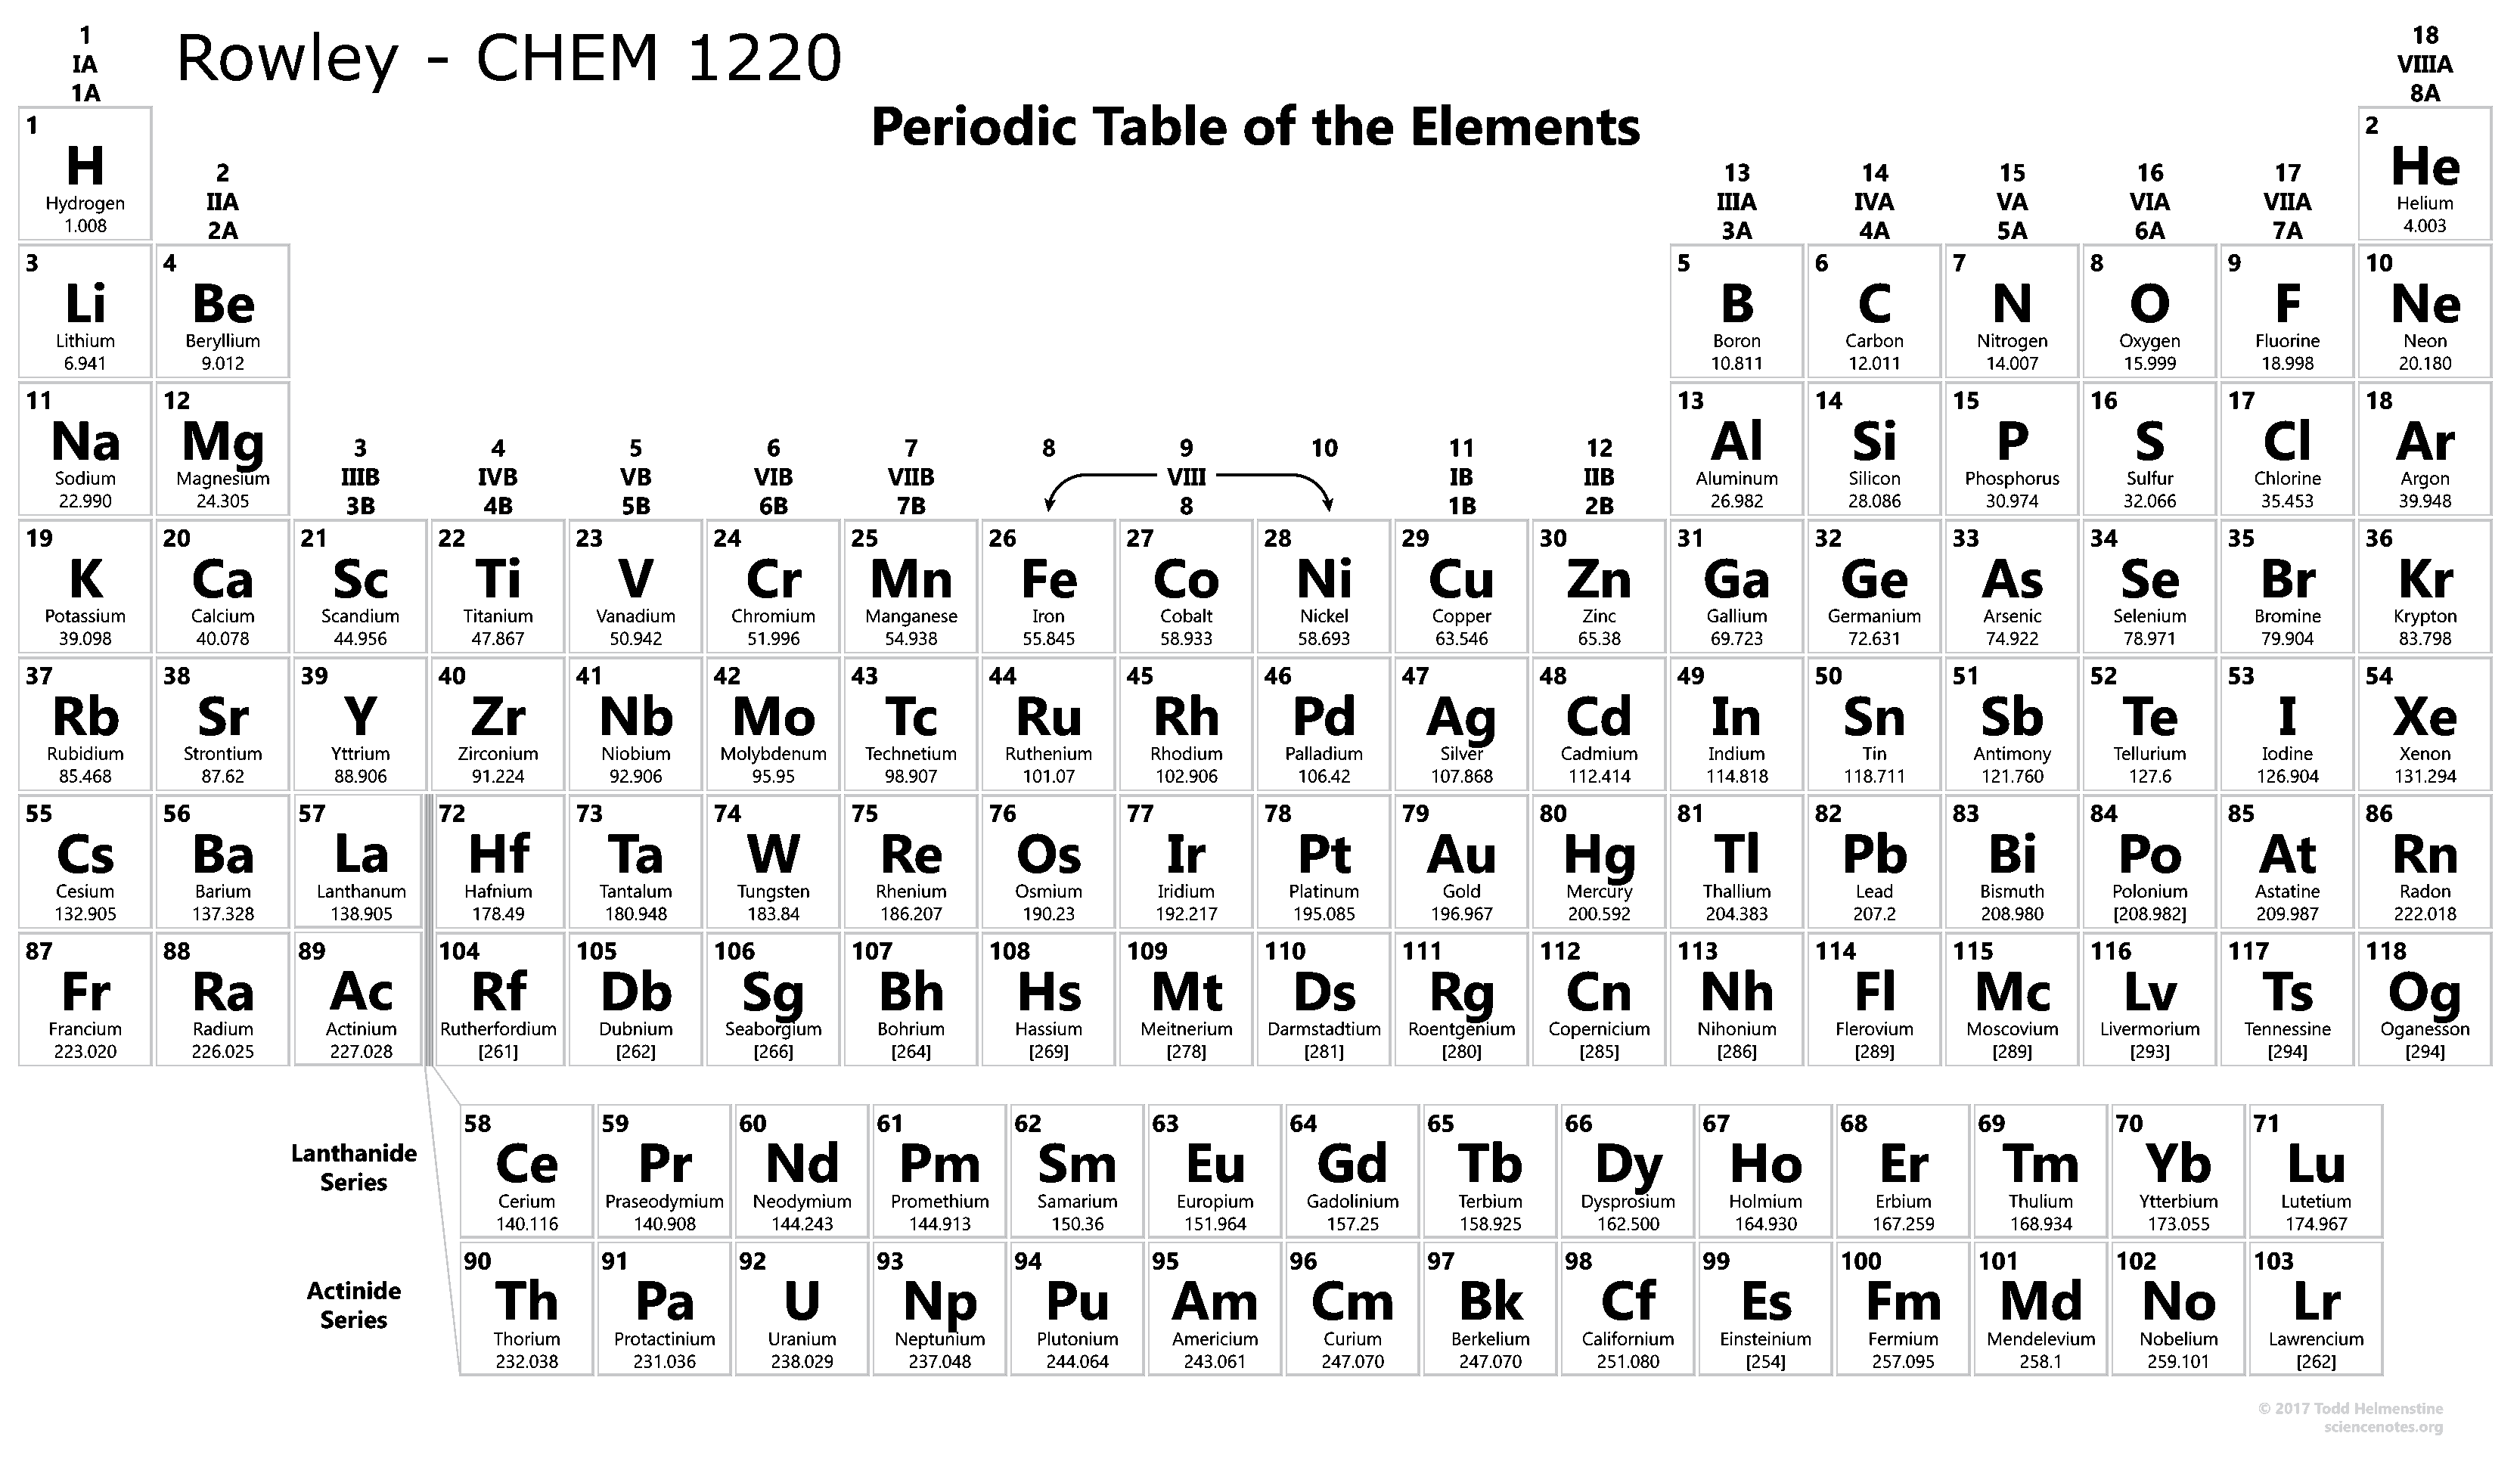
\includegraphics[width=1.3\textwidth, angle =90]{UpdatedTable.png}

	\restoregeometry

	
\end{document}